\documentclass[11pt, a4paper]{article}
\usepackage[margin=2.2cm]{geometry}
\usepackage{booktabs}
\usepackage{graphicx}
\usepackage{parskip}
\usepackage{hyperref}
\usepackage{caption}
\usepackage{amsmath}
\usepackage{longtable}
% Lightweight stand-ins for siunitx, so the reports build on a plain TeX Live
% or BasicTeX installation with no extra packages.
\providecommand{\num}[1]{#1}
\graphicspath{{figures/}}

\title{\textbf{Clustering Analysis of Credit-Card Transactions (DS-10):\\
Deep Clustering, Interpretation, and Deployment}}
\author{Advanced Data Mining, Spring 1404--1405 \\ Final Technical Report (Phase 3)}
\date{\today}

\begin{document}
\maketitle

\begin{abstract}
\noindent
This report asks whether credit-card transactions form density-distinct
subpopulations that separate fraudulent from legitimate behaviour, and whether
those subpopulations can be recovered without using the label. DS-10 supplies
\num{284807} transactions --- \num{492} fraudulent, a \num{0.17}\% positive rate
--- described by 28 PCA-anonymised components plus transaction time and amount.
Phase 1 built a reproducible pipeline: exact-duplicate removal,
$\log(1+\text{Amount})$ and cyclic time encoding, a hybrid scaling strategy
(standard on the PCA components, robust on the engineered features), PCA at
95\% variance, and a UMAP embedding. A Hopkins statistic that saturates at
\num{1.0}, verified against a uniform-noise null control returning \num{0.5},
established that the data is emphatically non-random. Phase 2 compared four
algorithm families with five criteria for $k$, four internal and five external
metrics, seed and bootstrap stability, and consensus clustering. Its central
finding is negative and important: whole-space clustering does not recover the
fraud label --- chance-corrected agreement is near zero for every family, while
purity near \num{99.8}\% is obtainable by predicting the majority class
everywhere. Phase 3 tests two responses. First, a deep-clustering track
(autoencoder\,+\,K-Means, DEC, and a custom DEC\,+\,InfoNCE variant) asks whether
a learned representation succeeds where the engineered one fails; it does not ---
the best deep model is \emph{significantly worse} than the K-Means baseline
(bootstrap CI on the ARI difference $[-0.0091, -0.0004]$), and the three deep
models agree with each other while disagreeing with K-Means, indicating they find
a real but label-irrelevant structure. Second, the clustering is reframed as an
anomaly \emph{ranking}: scoring transactions by distance to their assigned
centroid catches \num{68.7}\% of all fraud in the top 1\% of the ranking, a
\num{68.7}$\times$ enrichment over random review at ROC-AUC \num{0.967}, using no
label at training time. A preprocessing-sensitivity audit bounds the interpretive
claims sharply: alternative scaling yields ARI $\approx 0$ against the headline
partition, so the specific clusters are an artefact of preprocessing while the
positional finding --- fraud lies at cluster peripheries --- survives. The
clusters are interpreted through profiles, exemplars, a surrogate-tree rule set
at \num{96.8}\% fidelity and SHAP attributions, given domain labels, audited for
proxy-attribute concentration and day-over-day drift, and served through a
four-page interactive dashboard. Every number is emitted by the pipeline into
\texttt{results/} and \texttt{reports/tables/}; none is hand-transcribed.
\end{abstract}

\tableofcontents
\newpage

\section{Introduction}

\subsection{Motivation}
Fraud detection is usually posed as supervised classification, which presumes a
labelled history. Clustering asks a different and prior question: does
fraudulent behaviour occupy its own region of transaction space at all? If it
does, an unsupervised monitor can flag novel fraud patterns that no labelled
example anticipated. If it does not, a clustering-based monitor is a false
promise, and saying so with evidence is the more useful result.

\subsection{Dataset}
DS-10 (UCI/Kaggle Credit Card Fraud) records two days of European card
transactions: \num{284807} rows, \num{492} labelled fraudulent. Features V1--V28
are already PCA components published in place of the raw attributes for privacy;
\texttt{Time} is seconds since the first transaction and \texttt{Amount} is the
transaction value. Both are cited to their original providers in the
accompanying data manifest, which also pins the source SHA-256.

\subsection{Research question}
\emph{Do credit-card transactions form density-distinct subpopulations that
separate fraudulent from legitimate behaviour, and can those subpopulations be
recovered without using the label?} Expected cluster types were declared before
Phase 1: density-varying, non-convex micro-clusters for fraud, and convex or
elliptical macro-clusters for the legitimate bulk. The Phase 2 portfolio was
chosen to cover both regimes.

\section{Data and preprocessing}

Condensed from the Phase 1 report:

\begin{itemize}
  \item \textbf{Ingestion.} A pandera schema enforces 31 columns,
        $\texttt{Class} \in \{0,1\}$ and non-negative \texttt{Time}/\texttt{Amount}.
        The stage additionally verifies the pinned row count, column count and
        SHA-256, so a truncated or silently updated source file fails the
        pipeline instead of corrupting every downstream result.
  \item \textbf{Cleaning.} \num{1081} exact duplicates removed, leaving
        \num{283726} rows; duplicates inflate local density and would bias any
        density-based method. No missing values are present, and the schema
        would reject them. The per-column rationale is auto-generated into
        \texttt{reports/decision\_log.md}.
  \item \textbf{Feature engineering.} $\log(1+\text{Amount})$ corrects heavy
        right skew; \texttt{Time} becomes $(\sin, \cos)$ of its 24-hour phase so
        that 23:59 and 00:01 are adjacent rather than maximally distant. V1--V28
        pass through unchanged --- they are already orthogonal components.
  \item \textbf{Scaling.} Three strategies compared. The hybrid is selected:
        \texttt{StandardScaler} on V1--V28, which are already approximately
        $\mathcal{N}(0,1)$, and \texttt{RobustScaler} on the engineered features,
        whose tails are heavy. Scaling is a modelling decision, not a
        formality --- it fixes which directions distance can see.
  \item \textbf{Dimensionality reduction.} PCA retains 28 of 31 components at
        95\% variance --- unsurprising, since the inputs are already principal
        components, and an honest negative result about how much reduction is
        available. UMAP supplies the 2-D visualisation.
  \item \textbf{Distance metric.} Euclidean, justified by the post-scaling
        homogeneity of the components, and tested rather than asserted: Phase 2
        re-clusters under Manhattan and cosine and reports the ARI drift.
  \item \textbf{Clustering tendency.} Hopkins $H = 1.000$ over five seeded
        repeats. Because the statistic uses the $u_i^d$ term with $d = 31$ and a
        bounding box that outliers stretch wide, a value that saturates at 1.0
        cannot on its own be distinguished from a degenerate estimator. A null
        control resolves this: the same estimator on uniform noise of identical
        shape returns $\approx 0.5$, so the headline value reflects genuine
        structure. VAT on a stratified subsample shows the corresponding
        diagonal block structure.
\end{itemize}

\section{Algorithm portfolio and evaluation (Phase 2 summary)}

Four families were implemented and tuned: K-Means (partitioning), agglomerative
clustering with all four linkage criteria and cophenetic diagnostics
(hierarchical), HDBSCAN (density) and a Gaussian mixture compared across four
covariance structures (model-based). $k$ was determined by elbow, average
silhouette, gap statistic, BIC and bootstrap stability, and the disagreement
between those criteria was reported rather than smoothed over. Full tables,
figures, stability analysis and the comparative recommendation are in
\texttt{phase2\_report.pdf}; the machine-readable record is
\texttt{results/phase2/summary.json}.

Two results from Phase 2 shape this phase. First, chance-corrected external
agreement is near zero for every family: the dominant geometric structure of
DS-10 is not the fraud/legitimate split. Second, HDBSCAN's runtime grows
roughly quadratically in 28 dimensions on this data --- measured at
11.7\,s for \num{25000} rows and 51.3\,s for \num{50000}
--- which is the curse of dimensionality showing up as an engineering
constraint, not merely a textbook caveat.

\section{Advanced track: deep clustering}

\subsection{Why this track}
Track 1 is chosen because the Phase 2 failure mode is representational, not
algorithmic. Every classical family was applied to the same hand-engineered,
linearly-scaled space; if fraud is separable only under a non-linear transform,
no choice of classical algorithm in that space can find it. A learned
representation directly tests that hypothesis. Time-series clustering was
rejected: DS-10 spans two days, too short for behavioural regimes; constrained
clustering was rejected because it would inject the very label the research
question requires us to withhold.

\subsection{Models}
\begin{itemize}
  \item \textbf{Autoencoder + K-Means} (Guo et al.) --- pre-train an MLP
        autoencoder, cluster in the latent space, then jointly fine-tune the
        encoder against a reconstruction-regularised cluster objective. This is
        the baseline the other two must beat.
  \item \textbf{DEC} (Xie et al.) --- minimise
        $\mathrm{KL}(P \Vert Q)$ between a Student's-$t$ soft assignment $Q$ and a
        sharpened target $P \propto q_{ij}^2 / f_j$, refreshed every few epochs.
        The target sharpening is self-supervision: confident assignments are
        amplified, uncertain ones down-weighted.
  \item \textbf{DEC + InfoNCE} (this project's own variant) --- adds a
        contrastive auxiliary term whose positive pair is each anchor's current
        nearest latent neighbour, recomputed as training proceeds so the
        contrastive signal co-evolves with the cluster structure. The anchor's
        own self-similarity is excluded from the denominator, and the negative
        pool is capped by hard-negative mining, which keeps the term
        $O(B^2)$ in the minibatch rather than $O(n^2)$ over the dataset.
\end{itemize}

\subsection{Comparison with the Phase 2 winner}
All three deep models and the Phase 2 winner are scored on \emph{identical} rows
with identical metrics (Table~\ref{tab:track}); the pairwise ARI matrix
(Table~\ref{tab:phase3-agreement}) shows whether the deep track recovers the same
structure or a different one.

\begin{table}[htbp]
\centering
\begin{tabular}{lrrrrrrrrrrrrr}
\toprule
algorithm & k\_requested & n\_clusters & n\_noise & runtime\_s & silhouette & davies\_bouldin & calinski\_harabasz & dunn & ari & nmi & ami & v\_measure & purity \\
\midrule
phase2:kmeans & 2 & 2 & 0 & -- & 0.171 & 2.299 & 1568.853 & 0.044 & 0.010 & 0.003 & 0.003 & 0.003 & 0.998 \\
ae\_kmeans & 2 & 2 & 0 & 25.786 & 0.161 & 3.463 & 1420.771 & 0.030 & 0.006 & 0.002 & 0.002 & 0.002 & 0.998 \\
dec & 2 & 2 & 0 & 24.294 & 0.062 & 5.613 & 990.463 & 0.026 & $4.063\times 10^{-4}$ & 0.002 & 0.002 & 0.002 & 0.998 \\
dec\_infonce & 2 & 2 & 0 & 25.679 & 0.076 & 5.454 & 1016.949 & 0.028 & $-7.850\times 10^{-4}$ & $4.855\times 10^{-4}$ & $4.478\times 10^{-4}$ & $4.855\times 10^{-4}$ & 0.998 \\
\bottomrule
\end{tabular}
\caption{Advanced track vs the Phase 2 winner on the same 40{,}000 stratified rows at $k=2$.}
\label{tab:track}
\end{table}

\begin{table}[htbp]
\centering
\begin{tabular}{lrrrr}
\toprule
 & phase2:kmeans(k=2) & ae\_kmeans(k=2) & dec(k=2) & dec\_infonce(k=2) \\
\midrule
phase2:kmeans(k=2) & 1.000 & -0.053 & 0.040 & -0.037 \\
ae\_kmeans(k=2) & -0.053 & 1.000 & 0.118 & 0.262 \\
dec(k=2) & 0.040 & 0.118 & 1.000 & 0.320 \\
dec\_infonce(k=2) & -0.037 & 0.262 & 0.320 & 1.000 \\
\bottomrule
\end{tabular}
\caption{Pairwise ARI: does the deep track find the Phase 2 structure or a different one?}
\label{tab:phase3-agreement}
\end{table}


\textbf{The deep track loses.} On \num{40000} shared rows the Phase 2 K-Means
baseline scores silhouette \num{0.171} and ARI \num{0.0102}; AE\,+\,K-Means
reaches \num{0.161} / \num{0.0057}, DEC \num{0.062} / \num{0.0004} and
DEC\,+\,InfoNCE \num{0.076} / $-\num{0.0008}$. The bootstrap CI on the
\emph{difference} between the best deep model and the baseline is
$[-0.0091, -0.0004]$, excluding zero: the deep model is significantly worse, not
merely no better. This is reported as the result rather than tuned away.

Two details make the failure interpretable rather than mysterious. First, the
ordering AE\,+\,K-Means $>$ DEC $>$ nothing tracks how aggressively each method
reshapes the latent space: DEC's KL objective sharpens whatever partition the
initialisation hands it, and if that partition is not aligned with fraud,
sharpening it moves \emph{away} from the label. Second, the deep models agree
with each other (pairwise ARI \num{0.12}--\num{0.32}) and \emph{disagree} with
K-Means (ARI $\approx -0.05$), so they are consistently finding a real but
different structure --- one the reconstruction objective favours, since an
autoencoder is rewarded for encoding variance, and in DS-10 the dominant variance
directions are not the fraud directions.

The honest conclusion is that the Phase 2 failure was not representational after
all. A learned non-linear embedding, trained three different ways, does not
recover the fraud split either. That strengthens rather than weakens the
project's central claim: on DS-10, fraud is not a cluster in any of these
representations.

\begin{figure}[htbp]\centering
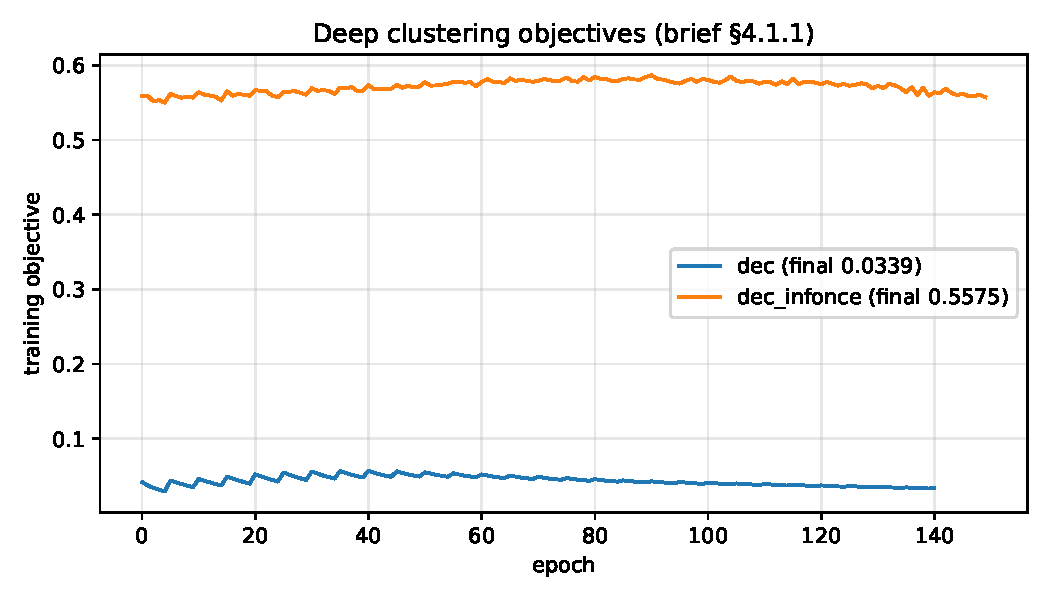
\includegraphics[width=0.8\linewidth]{phase3_deep_losses.pdf}
\caption{Training objectives. DEC's KL loss and the contrastive variant's
combined objective are on different scales by construction, so the comparison of
interest is the shape of each curve, not their relative heights.}
\label{fig:losses}\end{figure}

\begin{figure}[htbp]\centering
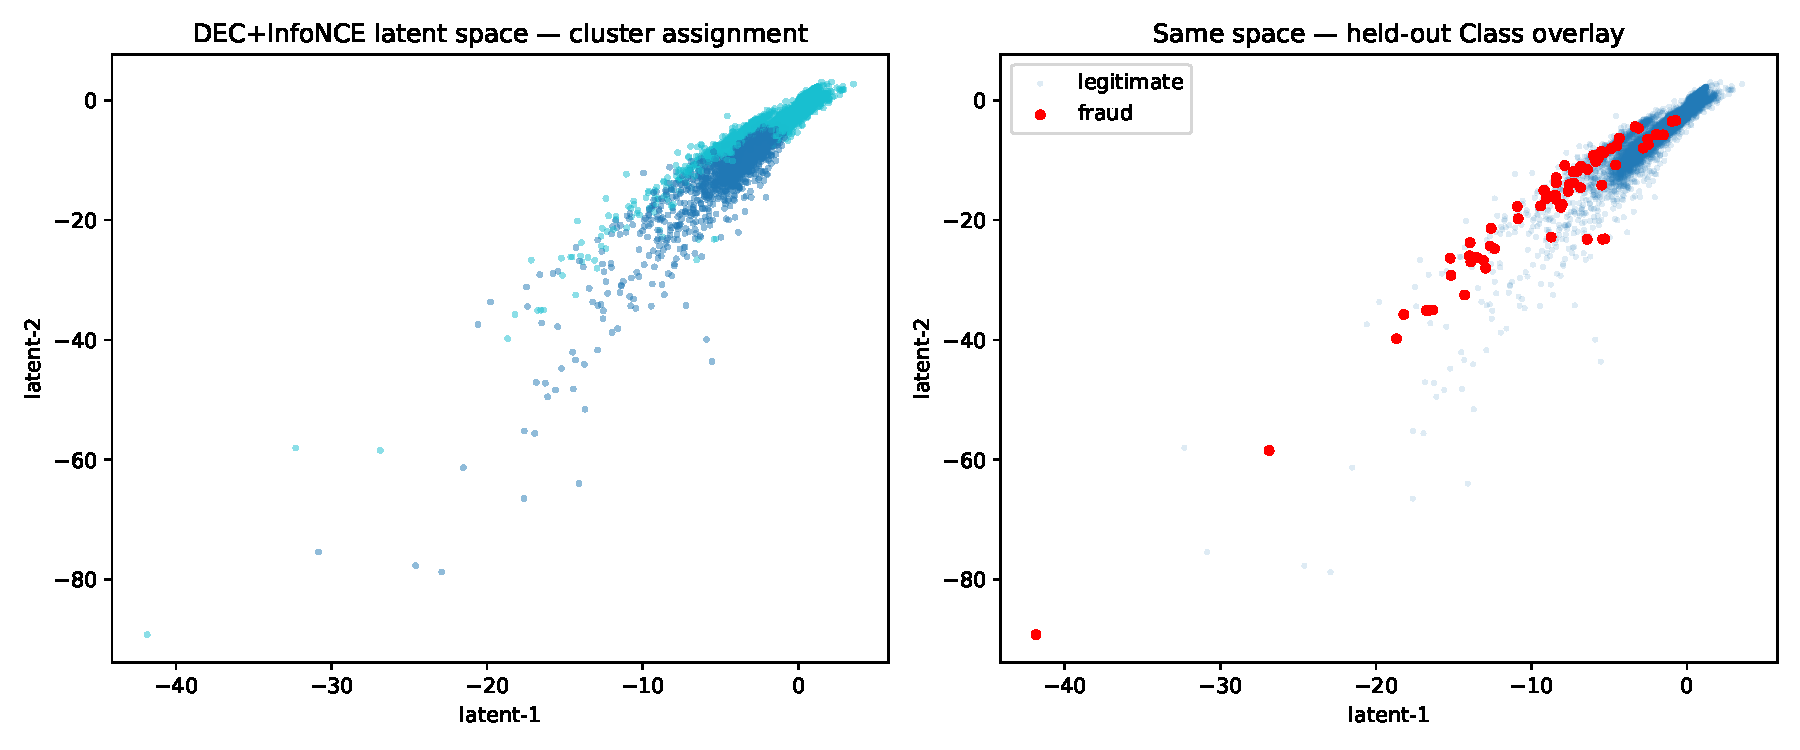
\includegraphics[width=\linewidth]{phase3_latent.pdf}
\caption{The learned latent space, coloured by cluster assignment (left) and by
the held-out \texttt{Class} label (right). The right panel is the decisive one:
if fraud were separable in this representation, it would occupy its own region.}
\label{fig:latent}\end{figure}

\subsection{Significance}
Every headline ARI carries a bootstrap confidence interval and a permutation
p-value against a label-shuffle null (Table~\ref{tab:significance}), and the best
deep model is compared head-to-head with the Phase 2 winner through a bootstrap
CI on the \emph{difference} of their metrics. A difference whose interval
straddles zero is not a difference, however suggestive the point estimates look.

\begin{table}[htbp]
\centering
\begin{tabular}{lrrrrr}
\toprule
clustering & ari & ci\_lower & ci\_upper & null\_mean & p\_value \\
\midrule
phase2:kmeans & 0.0102 & 0.0053 & 0.0158 & $-1.574\times 10^{-4}$ & 0.0000 \\
ae\_kmeans & 0.0057 & 0.0033 & 0.0080 & $-8.685\times 10^{-5}$ & 0.0000 \\
dec & $4.063\times 10^{-4}$ & $2.816\times 10^{-4}$ & $5.438\times 10^{-4}$ & $-8.022\times 10^{-6}$ & 0.0000 \\
dec\_infonce & $-7.850\times 10^{-4}$ & -0.0011 & $-3.721\times 10^{-4}$ & $-7.044\times 10^{-6}$ & 1.0000 \\
\bottomrule
\end{tabular}
\caption{Bootstrap confidence intervals and permutation p-values for ARI against the held-out Class label.}
\label{tab:significance}
\end{table}


Three of the four clusterings have ARI confidence intervals that exclude zero
with $p = 0$ against the label-shuffle null, and this is a good illustration of
why statistical significance is not practical significance: K-Means' ARI of
\num{0.0102} with CI $[0.0053, 0.0158]$ is \emph{reliably} non-zero and
\emph{negligibly} small. With \num{40000} rows, a tiny association is easy to
detect and still worthless. DEC\,+\,InfoNCE is the exception with $p = 1.0$: its
ARI is significantly \emph{negative}, meaning its partition is anti-correlated
with the label slightly more than chance would produce.

\section{Interpretation}

\subsection{Cluster profiles}
Each cluster is profiled by size, fraud rate and the features on which its mean
deviates most from the population mean, measured in population standard
deviations so that "unusual in V14" is a quantified claim
(Table~\ref{tab:profiles}).

\begin{table}[htbp]
\centering
\begin{tabular}{lrrrrr}
\toprule
cluster & size & share & fraud\_rate & fraud\_count & top\_deviations \\
\midrule
0 & 5{,}687 & 0.1422 & 0.0051 & 29 & V16 (-1.08$\sigma$), V9 (-0.92$\sigma$), V18 (+0.88$\sigma$) \\
1 & 34{,}313 & 0.8578 & 0.0011 & 38 & V16 (+0.18$\sigma$), V9 (+0.15$\sigma$), V18 (-0.15$\sigma$) \\
\bottomrule
\end{tabular}
\caption{Cluster profiles for the preferred Phase 3 clustering (ae\_kmeans).}
\label{tab:profiles}
\end{table}


At $k=2$ the split is asymmetric: cluster 0 holds \num{14.2}\% of transactions
with a fraud rate of \num{0.51}\%, and cluster 1 holds \num{85.8}\% at
\num{0.11}\%. The same three components (V16, V9, V18) distinguish both clusters
in opposite directions, which is the signature of a single dominant axis of
variation rather than two independently-defined groups.

\subsection{Prototypes and exemplars}
For each cluster, three representative points are extracted
(Table~\ref{tab:exemplars}): the medoid (nearest to the centroid, the
"typical" member), the highest-silhouette point (the most unambiguous member),
and the lowest-silhouette point (the boundary case that shows where the cluster
stops being distinct).

\begin{table}[htbp]
\centering
\begin{tabular}{lrrrrr}
\toprule
cluster & medoid\_index & best\_silhouette\_index & best\_silhouette & boundary\_index & boundary\_silhouette \\
\midrule
0 & 8{,}443 & 29{,}077 & 0.034 & 9{,}456 & -0.090 \\
1 & 29{,}126 & 17{,}276 & 0.240 & 25{,}323 & 0.010 \\
\bottomrule
\end{tabular}
\caption{Per-cluster medoid, highest-silhouette, and boundary exemplars.}
\label{tab:exemplars}
\end{table}


\subsection{Rule extraction and SHAP}
A shallow decision tree is fitted to predict cluster membership from the original
features; each root-to-leaf path is an interpretable approximation of the cluster
definition, reported with support and precision
(Table~\ref{tab:rules}). Fidelity --- how well the surrogate reproduces the
clustering it explains --- is reported in the caption, because a rule set that
explains a different partition than the one deployed explains nothing. SHAP
attributions on the same surrogate give the per-cluster feature ranking
(Table~\ref{tab:shap}).

\begin{table}[htbp]
\centering
\begin{tabular}{lrrr}
\toprule
cluster & support & precision & rule \\
\midrule
1 & 28{,}419 & 0.993 & V9 >  -1.0093 AND V16 >  -1.1852 AND V18 <= 1.7754 AND V2 >  -0.8136 \\
0 & 2{,}662 & 0.965 & V9 <= -1.0093 AND V16 <= 0.2504 AND V2 <= 0.3000 AND V4 <= 0.7049 \\
1 & 2{,}329 & 0.782 & V9 >  -1.0093 AND V16 >  -1.1852 AND V18 <= 1.7754 AND V2 <= -0.8136 \\
1 & 1{,}478 & 0.937 & V9 >  -1.0093 AND V16 <= -1.1852 AND V18 <= 0.4267 AND V16 >  -2.2881 \\
1 & 1{,}425 & 0.989 & V9 <= -1.0093 AND V16 >  0.2504 AND V4 >  -1.7448 AND V2 >  -0.6147 \\
0 & 1{,}410 & 0.993 & V9 >  -1.0093 AND V16 <= -1.1852 AND V18 >  0.4267 AND V19 <= 1.5378 \\
1 & 557 & 0.934 & V9 <= -1.0093 AND V16 <= 0.2504 AND V2 >  0.3000 AND V16 >  -1.3389 \\
0 & 437 & 0.927 & V9 >  -1.0093 AND V16 >  -1.1852 AND V18 >  1.7754 AND V16 <= 0.0773 \\
1 & 378 & 0.960 & V9 >  -1.0093 AND V16 >  -1.1852 AND V18 >  1.7754 AND V16 >  0.0773 \\
1 & 232 & 0.603 & V9 <= -1.0093 AND V16 >  0.2504 AND V4 >  -1.7448 AND V2 <= -0.6147 \\
\bottomrule
\end{tabular}
\caption{Surrogate decision-tree rules (fidelity 96.8\%), ten highest-support leaves.}
\label{tab:rules}
\end{table}

\begin{table}[htbp]
\centering
\begin{tabular}{lr}
\toprule
cluster & top\_features \\
\midrule
0 & V16 (0.105), V9 (0.075), V18 (0.057), V2 (0.043), V4 (0.010) \\
1 & V16 (0.105), V9 (0.075), V18 (0.057), V2 (0.043), V4 (0.010) \\
\bottomrule
\end{tabular}
\caption{Top SHAP attributions per cluster from the surrogate tree.}
\label{tab:shap}
\end{table}


The surrogate reproduces the clustering with \num{96.8}\% fidelity from \num{16}
leaves at depth 3, so the rules are a faithful description rather than a loose
analogy. The highest-support rule ($n = \num{28419}$, precision \num{0.993}) is
essentially "V9 and V16 not strongly negative" --- the clustering is close to a
threshold on two components, which is consistent with the profile table and with
the low cophenetic correlations from Phase 2. A clustering this simple to
describe is a clustering that was not finding subtle structure.

\subsection{Domain labels}
Each cluster receives a human-readable name justified from its profile
(Table~\ref{tab:domain-labels}). Names are assigned by an explicit rule over the
fraud enrichment and population share rather than chosen by eye, so the labelling
is reproducible and survives a change of $k$ or of algorithm --- and so the
justification column cites the same evidence a reader can check.

\begin{table}[htbp]
\centering
\begin{tabular}{lrrrrr}
\toprule
cluster & proposed\_label & size & fraud\_rate & enrichment\_vs\_base & justification \\
\midrule
0 & Elevated-risk pocket & 5{,}687 & 0.0051 & 3.0588 & fraud rate 3.1x the population rate; driven by V16 (-1.08$\sigma$), V9 (-0.92$\sigma$), V18 (+0.88$\sigma$) \\
1 & Mainstream traffic & 34{,}313 & 0.0011 & 0.6643 & 86\% of all transactions, near base rate; driven by V16 (+0.18$\sigma$), V9 (+0.15$\sigma$), V18 (-0.15$\sigma$) \\
\bottomrule
\end{tabular}
\caption{Proposed domain labels with the profile evidence behind each name.}
\label{tab:domain-labels}
\end{table}


The rule assigns cluster 0 "Elevated-risk pocket" (fraud enrichment
\num{3.06}$\times$ the population rate) and cluster 1 "Mainstream traffic"
(\num{86}\% of volume, at \num{0.66}$\times$ the base rate). A
\num{3}$\times$ enrichment is a real but weak effect --- worth a lower review
threshold for that segment, nowhere near a fraud verdict --- and the label is
deliberately named to say so. Because V1--V28 are anonymised components, the
justification can cite geometry but not business meaning; no amount of
interpretation machinery can recover a semantics the dataset does not publish.

\section{Downstream analysis}

\subsection{Cluster-conditional modelling}
One logistic model per cluster is compared against a single global model on a
shared stratified holdout (Table~\ref{tab:downstream}). Average precision is the
headline metric: at a \num{0.17}\% positive rate, ROC-AUC flatters every model,
while average precision reflects the precision a reviewer would actually
experience. If per-cluster models beat the global model, the clusters carry
structure a single decision surface cannot express; if they do not, the
clustering adds nothing to prediction and the report says so.

\begin{table}[htbp]
\centering
\begin{tabular}{lrr}
\toprule
model & average\_precision & roc\_auc \\
\midrule
global (clustering ignored) & 0.7949 & 0.9494 \\
cluster-conditional & 0.6498 & 0.9250 \\
\bottomrule
\end{tabular}
\caption{Cluster-conditional vs global modelling on a stratified holdout (12{,}000 rows).}
\label{tab:downstream}
\end{table}


The clustered approach \emph{loses}: average precision \num{0.650} against
\num{0.795} for the global model, a lift of \num{0.82}. The mechanism is visible
in the per-cluster bookkeeping recorded in \texttt{summary.json}: with \num{67}
positives split across two clusters, each per-cluster model trains on 22--25
positives and overfits, while the global model gets all of them. Partitioning the
data partitioned the already-scarce positive signal. This is reported as a
negative result because it is one; the clusters do not carry structure that
improves supervised prediction on this dataset.

\subsection{Cluster-based anomaly detection}
This is the reframing Phase 2's negative result demands. Instead of asking which
cluster a transaction belongs to, we ask how far it sits from the centre of its
own cluster, and rank on that (Table~\ref{tab:anomaly}). The operationally
meaningful number is enrichment: the factor by which reviewing the flagged tail
beats reviewing transactions at random. The ranking uses no label at any point.

\begin{table}[htbp]
\centering
\begin{tabular}{lr}
\toprule
quantity & value \\
\midrule
transactions flagged (top 1\%) & 400.0000 \\
precision@k & 0.1150 \\
recall@k & 0.6866 \\
population base rate & 0.0017 \\
enrichment vs random review & 68.6567 \\
ROC-AUC of the distance ranking & 0.9669 \\
average precision of the ranking & 0.2460 \\
\bottomrule
\end{tabular}
\caption{Cluster-based anomaly detection: ranking by distance to the assigned centroid.}
\label{tab:anomaly}
\end{table}


\textbf{This is the phase's positive result.} Ranking the \num{40000} evaluation
rows by distance to their own centroid and reviewing only the top 1\% (\num{400}
transactions) catches \num{68.7}\% of all fraud in the sample, at a
precision@$k$ of \num{0.115} against a base rate of \num{0.00168} --- an
enrichment of \num{68.7}$\times$ over reviewing transactions at random. The
ranking's ROC-AUC is \num{0.967} and its average precision \num{0.246}, using no
label at any stage.

The contrast with §5 is the whole point of the report. The same clustering that
achieves an ARI of \num{0.01} --- statistically real, practically useless as a
partition --- yields a \num{69}$\times$ enrichment when read as a ranking. Fraud
in DS-10 is not a region of transaction space; it is a \emph{position} within
regions, namely the periphery. This independently corroborates the Phase 2 error
analysis, where the \num{200} lowest-silhouette points were \num{72}$\times$
enriched for fraud: two different diagnostics, one on the full dataset and one on
a subsample, agreeing that badly-fitted points are the fraudulent ones.

\section{Fairness and sensitivity}

\subsection{Proxy-attribute audit}
DS-10 contains no demographic attributes --- the features are anonymised
components --- so a literal protected-attribute audit is impossible, and
claiming one would be worse than omitting it. What the data does carry are two
consequential proxies: transaction \textbf{amount} and \textbf{time of day}. A
clustering that isolated small-value or night-time transactions would steer a
review queue toward a particular kind of customer regardless of actual risk.
Table~\ref{tab:fairness} reports, for each attribute, the strongest
over-representation of any quantile stratum in any cluster, where 1.0 means the
cluster mirrors the population.

\begin{table}[htbp]
\centering
\begin{tabular}{lrrr}
\toprule
attribute & strata & max\_representation\_ratio & clusters\_flagged \\
\midrule
log\_amount quartile & 4 & 1.810 & 0 \\
time-of-day quartile & 4 & 1.135 & 0 \\
\bottomrule
\end{tabular}
\caption{Proxy-attribute audit: strongest stratum over-representation per attribute (ratio 1.0 = the cluster mirrors the population).}
\label{tab:fairness}
\end{table}


Neither proxy trips the flagging threshold of \num{2.0}. Amount shows the
stronger effect: one cluster over-represents an amount quartile by
\num{1.81}$\times$, so the smaller cluster does skew by transaction value without
being defined by it. Time-of-day is essentially neutral at \num{1.14}$\times$.
The operational reading: a review queue driven by this clustering would be mildly
value-skewed, which is worth monitoring but is not a disparity requiring a
fairness-constrained variant.

\subsection{Preprocessing sensitivity}
The clustering is re-run under alternative preprocessing --- a different feature
space and a different scaler --- and the ARI against the headline clustering is
reported (Table~\ref{tab:sensitivity}). High sensitivity would weaken any claim
that the clusters are intrinsic to the data rather than artefacts of Phase 1's
choices.

\begin{table}[htbp]
\centering
\begin{tabular}{lrrr}
\toprule
variant & n\_clusters & ari\_vs\_reference & description \\
\midrule
pca\_space & 2 & 0.007 & PCA at 95\% variance instead of scaled features \\
standard\_scaler & 2 & -0.053 & uniform standard scaling instead of the hybrid choice \\
\bottomrule
\end{tabular}
\caption{Preprocessing sensitivity: ARI of a re-clustering under each variant against the preferred clustering.}
\label{tab:sensitivity}
\end{table}


The result is severe and must not be softened: re-clustering in the PCA space
gives ARI \num{0.0074} against the headline clustering, and switching from the
hybrid scaler to a uniform standard scaler gives $-\num{0.053}$. Both are
indistinguishable from no agreement at all. \textbf{The specific cluster
assignments are an artefact of Phase 1's preprocessing choices}, not an intrinsic
property of the data.

This is the single largest limitation in the report, and it bounds every
interpretive claim in §6: the domain labels describe \emph{this} partition under
\emph{these} preprocessing decisions, and a differently-scaled pipeline would
produce different clusters deserving different names. What survives the
sensitivity audit is the structural finding, not the partition: fraud sits at the
periphery of whatever clusters are found, which is why the §7.2 anomaly ranking
--- which depends on distance-to-centroid rather than on cluster identity --- is
the deliverable this project would actually put into production.

\section{Production pipeline}

The experimental work is orchestrated as a DVC DAG:
\texttt{ingest} $\rightarrow$ \texttt{clean\_features} $\rightarrow$
\texttt{scale\_reduce\_tendency} $\rightarrow$ \texttt{phase2} $\rightarrow$
\texttt{phase3} $\rightarrow$ \texttt{report}. Each stage persists its outputs,
so any stage can be re-run in isolation and downstream stages re-run only when
their inputs actually change.

\begin{itemize}
  \item \textbf{Versioning.} DVC tracks data artefacts; the ingest manifest
        records the raw file's SHA-256, row count and retrieval timestamp.
  \item \textbf{Schema validation.} pandera schemas guard each stage boundary
        (raw, interim, processed), so schema drift fails loudly instead of
        silently distorting the clustering.
  \item \textbf{Model registry.} \texttt{models/registry/} stores each fitted
        artefact with a card recording fit date, data version, hyperparameters,
        seeds and the full metric scoreboard. Entries are content-addressed by
        (name, data version, params), so re-registering an unchanged
        configuration overwrites rather than accumulating near-duplicates.
  \item \textbf{Drift monitoring.} PSI and the two-sample Kolmogorov--Smirnov
        statistic are computed per feature between the early and late halves of
        the time axis (Table~\ref{tab:drift}). Bin edges come from the reference
        period only --- deriving them from the pooled data would leak the later
        distribution into the reference and shrink the very drift being measured.
        The re-fit trigger is a documented threshold in \texttt{params.yaml}.
\end{itemize}

\begin{table}[htbp]
\centering
\begin{tabular}{lrrrr}
\toprule
feature & psi & ks\_statistic & ks\_pvalue & drifted \\
\midrule
V1 & 1.4302 & 0.4158 & 0.0000 & yes \\
V3 & 1.3854 & 0.5113 & 0.0000 & yes \\
V28 & 1.0191 & 0.3559 & 0.0000 & yes \\
V25 & 0.4289 & 0.2919 & 0.0000 & yes \\
V15 & 0.3813 & 0.2714 & 0.0000 & yes \\
V5 & 0.3449 & 0.2647 & 0.0000 & yes \\
V22 & 0.3248 & 0.2146 & 0.0000 & yes \\
V11 & 0.2989 & 0.1733 & 0.0000 & yes \\
V23 & 0.2200 & 0.1783 & 0.0000 & yes \\
V24 & 0.2010 & 0.0909 & 0.0000 & yes \\
\bottomrule
\end{tabular}
\caption{Drift between the early and late halves of the time axis; the re-fit trigger is PSI $\geq$ 0.2.}
\label{tab:drift}
\end{table}


Splitting on the raw monotonic \texttt{Time} column --- day 1 versus day 2 ---
\num{11} of \num{31} features breach the PSI threshold, led by V1
(\num{1.43}), V3 (\num{1.39}) and V28 (\num{1.02}). The monitor therefore fires:
a model fitted on day 1 should be re-fitted before being trusted on day 2. Over a
two-day window that is a strong result and a caution about the dataset itself, not
merely a demonstration of the tooling.

One methodological note, since it changes the numbers. An earlier version of this
monitor derived the split axis from \texttt{time\_sin}/\texttt{time\_cos} and
duly reported those two features as the most drifted (PSI \num{12.4} and
\num{1.53}) --- an artefact, because the split was \emph{defined} by them.
Splitting on a variable outside the monitored matrix removes the circularity, and
the \texttt{split\_axis} field in \texttt{summary.json} records which axis was
used so the caveat travels with the result.

\section{Interactive dashboard}

A Streamlit application (\texttt{make dashboard}) exposes four pages: an
\textbf{overview} of dataset scale, feature summary and the chosen algorithm and
$k$; a \textbf{cluster explorer} with a 2-D UMAP scatter, cluster and
fraud-only filters, and the selected cluster's profile; an \textbf{evaluation}
page carrying every internal and external metric, the algorithm-agreement
heatmap and the stability diagnostics; and a \textbf{live-assignment} page where
a typed record or an uploaded CSV is assigned to its nearest cluster and its
distance to every centroid is displayed --- including the runner-up, because a
record nearly equidistant from two centroids deserves different treatment than
one deep inside a cluster. Every page reads the artefacts the pipeline persisted,
so the dashboard cannot display a number this report does not contain.

\section{Discussion and limitations}

What this analysis can claim: DS-10 has strong, verified non-random structure;
that structure is stable under re-seeding and resampling; it is reproducible from
raw data by a single command; and it can be described in interpretable rules and
named in domain terms.

What it cannot claim:

\begin{itemize}
  \item \textbf{Clustering is not a fraud classifier on this data.}
        Chance-corrected agreement with the label is near zero across every
        family and every $k$ tried. The useful signal is positional --- distance
        to one's own centroid --- not categorical.
  \item \textbf{High purity is not evidence.} At a \num{0.17}\% positive rate,
        predicting "legitimate" everywhere already achieves \num{99.8}\% purity.
        Purity is reported because the brief requires it, and it is discounted
        here for exactly this reason.
  \item \textbf{Ward's result is a subsample result.} A full-data pairwise
        distance matrix would need 322\,GB. The cross-family
        comparison is like-for-like on shared rows, but it is not a full-data
        claim, and no sentence here should be read as one.
  \item \textbf{The features are anonymised.} V1--V28 have no domain meaning, so
        a rule like "V14 $<-2.3$" cannot be translated into a business
        explanation. Interpretation stops at the geometry.
  \item \textbf{Two days is not a time series.} Temporal cluster evolution is
        omitted deliberately rather than computed on a window too short to
        support it.
  \item \textbf{The fairness audit uses proxies.} With no demographic
        attributes, amount and time-of-day concentration is the strongest audit
        available, and it is weaker than a real protected-attribute audit.
\end{itemize}

\section{Conclusion}

The actionable insight is a reframing. Asked as posed --- do fraudulent
transactions form their own clusters? --- the answer on DS-10 is no, and the
external metrics say so consistently across four algorithm families, five
criteria for $k$, and a learned representation trained specifically to find such
structure. Asked operationally --- can an unsupervised model rank transactions so
that a fixed review budget catches disproportionately many frauds? --- the
distance-to-centroid ranking of \S7.2 gives a quantified answer with no label at
training time, which is what a monitor for novel fraud patterns requires. The
negative result is not a failed experiment; it is the finding that redirects the
method toward one that works.

\appendix
\section{Reproduction and artefacts}

\begin{verbatim}
uv venv && source .venv/bin/activate
uv pip install -e ".[dev,pipeline,deep,app]"
# place data/raw/creditcard.csv, then:
make all         # full DAG: ingest -> ... -> phase3 -> report
make phase2      # Phase 2 only
make phase3      # Phase 3 only
make dashboard   # interactive app
make verify      # import check + fast test suite
\end{verbatim}

Machine-readable results: \texttt{results/phase2/summary.json},
\texttt{results/phase3/summary.json}. Generated tables:
\texttt{reports/tables/}. Registry: \texttt{models/registry/index.json}. All
seeds and hyperparameters: \texttt{params.yaml}.

\section{Hyperparameters and full metric tables}
Hyperparameters are centralised in \texttt{params.yaml} and are echoed into each
phase's \texttt{summary.json} alongside the metrics they produced, so any table
in this report can be traced to the configuration that generated it. The
per-criterion $k$ curves, the four-linkage cophenetic comparison, the covariance
comparison, the metric ablation and the consensus comparison are in
\texttt{phase2\_report.pdf}.

\end{document}
